\documentclass[a4paper]{article}
\usepackage[big]{layaureo}
\usepackage{verbatim}
\usepackage{color}
\usepackage{listings}
\usepackage{graphicx}

\title{Relazione del progetto del Laboratorio di Applicazioni Internet}
\author{Federico Mariti}

\begin{document}

\maketitle

\section{Descrizione del problema}
\label{sec:descrizione}
Un albergo richiede la pubblicazione di due funzionalit\`a: la ricerca
di una camera e la prenotazione di una camera. Una camera dell'albergo
\`e caratterizzata dalle seguenti propriet\`a:
\begin{itemize}
\item il numero massimo di persone adulte e di bambini che
  pu\`o ospitare, 
\item da un codice che identifica la tipologia della stanza, ad
  esempio matrimoniale, doppia, suite, etc ...,
\item il costo per notte,
\item un elenco dei servizi disponibili,
\item un codice identificativo usato dall'albergo per riferirsi
  unicamente a tutte quelle stanze che rispettino le proprit\`a
  precedenti,
\item il numero di stanze con stesso identificatore diposonibili
  nell'albergo.
\end{itemize}
La ricerca di una stanza pu\`o essere effettuata specificando, oltre
ad un periodo temporale, il numero di adulti e di bambini; per
raffinare la ricerca possono essere aggiunte le altre propriet\`a di
una stanza. La prenotazione di una stanza richiede, oltre che ad un
periodo temporale, il codice identificativo con cui l'albergo
riferisce alla stanza, e le informazioni sugli ospiti e sulla carta di
credito con cui effettuare il pagamento. La prenotazione viene
registarata con stanto ``pendente'' se la stanza specificata \`e
disponibile per il periodo temporale specificato, successivamente con
stato ``confermato'' a pagamento avvenuto. La prenotazione non viene
registrata se non viene fornito l'identificatore della stanza (la
richiesta \`e ambigua) o se la stanza specificata non \`e disponibile
nel periodo di tempo specificato.

%%%%%%%%%%%%%%%%%%%%%%%%%%%%%%%%%%%%%%%%%%%%%%%%%%%%%%%%%%%%%%%%%%%%%%%%%%%%%

\section{Le specifiche richieste dal progetto}
Di seguito viene spiegato come sono state realizzate le specifiche
richieste:
\begin{itemize}
\item I due web service richiesti realizzano rispettivamente le
  funzionalit\`a di ricerca di una stanza e di prenotazione di una
  stanza, sono descritti nei file WSDL \verb'WebContent/ricerc'\-\verb'a.wsdl'
  e \verb'WebContent/prenotazione.wsdl'. Per brevit\`a, nel seguito,
  verranno chiamati \emph{ricerca-ws} e \emph{prenotazione-ws}.
\item Di fatto l'approccio con cui si sono implementati entrambi i web
  service \`e stato quello \emph{Top-Down}, ovvero per entrambi i web
  service si \`e partiti dalla definizione delle descrizioni WSDL,
  dopo di che si \`e implementato le funzionalit\`a in Java. Sono
  stati usati gli strumenti forniti dal framework Apache CXF:
  \begin{itemize}
    \item \`e stata usata l'utility \verb'wsdl2java' per creare le
      classi skeleton del \emph{prenotazione-ws}, l'implementazione
      della logica applicativa di tale web service prevede quindi
      l'uso di oggetti delle classi Java create,
    \item il \emph{ricerca-ws} ha tutte le funzionalit\`a realizzate
      nel metodo \verb'invoke' di una classe Java che implementa
      l'interfaccia \verb'javax.xml.ws.Provider<SOAPMessage>', per
      tanto l'implementazione della logica applicativa prevede la
      gestione manuale dei messaggi SOAP, ci\`o \`e stato realizzato
      con le sole funzionalit\`a della SAAJ.
  \end{itemize}
\item Entrambi i web service interagiscono con il database
  dell'hotel per l'espletazione delle funzionalit\`a.
\item Tutte le comunicazioni utilizzano il protocollo HTTP per il
  trasporto delle informazioni. In alcune interazioni vengono
  realizzati dei livelli di sicurezza per mezzo della PKI X.509:
  \begin{itemize}
  \item tutti i messaggi di risposta inviati dai web service ai
    client sono firmati,
  \item nel messaggio di richista di prenotazione di una stanza le
    informazioni relative alla carta di credito sono cifrate.
  \end{itemize}
\item Il componenete applicativo Proxy \`e realizzato con una Servlet
  Java, l'analisi dei messaggi SOAP ricevuti viene effettuata
  unicamente con le funzionalit\`a della JAX-P. Tale componente
  realizza anche la validazione del contenuto SOAP e del contenuto
  appplicativo (se non \`e cifrato) dei messaggi di richiesta ricevuti
  dai client.
\item \`E stato realizzato un programma Java che agisce da cliente
  dell'applicazione e che interagisce con il Proxy. Tale programma \`e
  state-less e comandato da agromenti da riga di comando. Viene usato
  il framework Spring per la specifica WS-S.
\end{itemize}

%%%%%%%%%%%%%%%%%%%%%%%%%%%%%%%%%%%%%%%%%%%%%%%%%%%%%%%%%%%%%%%%%%%%%%%%%%%%%

\section{Messaggi SOAP e schemi XML}
\label{sec:xml}
Si \`e adottato l'approccio \emph{Top-Down} per l'implementazione dei
servizi, perci\`o si \`e defito, prima di tutto, lo schema XML
dell'applicazione, quindi si \`e data la descrizione dei web services,
tramite due file WSDL, poi si \`e realizzata l'implementazione Java.

La definizione dello schema XML dell'applicazione \`e divisa in tre
file XSD: uno di questi \`e \verb+hotel.xsd+ e defisce i tipi di dato
generali, usati da entrambi i web service dell'applicazione, gli altri
due file XSD sono \verb+ricerca.xsd+ e \verb+prenotazione.xsd+, si
riferiscono ad uno specifico web service, includono \verb+hotel.xsd+ e
definiscono i tipi e gli elementi propri del corrispondente web
service. Nella figura \ref{tipiXSD-figura} sono mostrati, in modo
informale, i principali tipi di dato definiti nei file XSD.

\begin{figure}[h]
  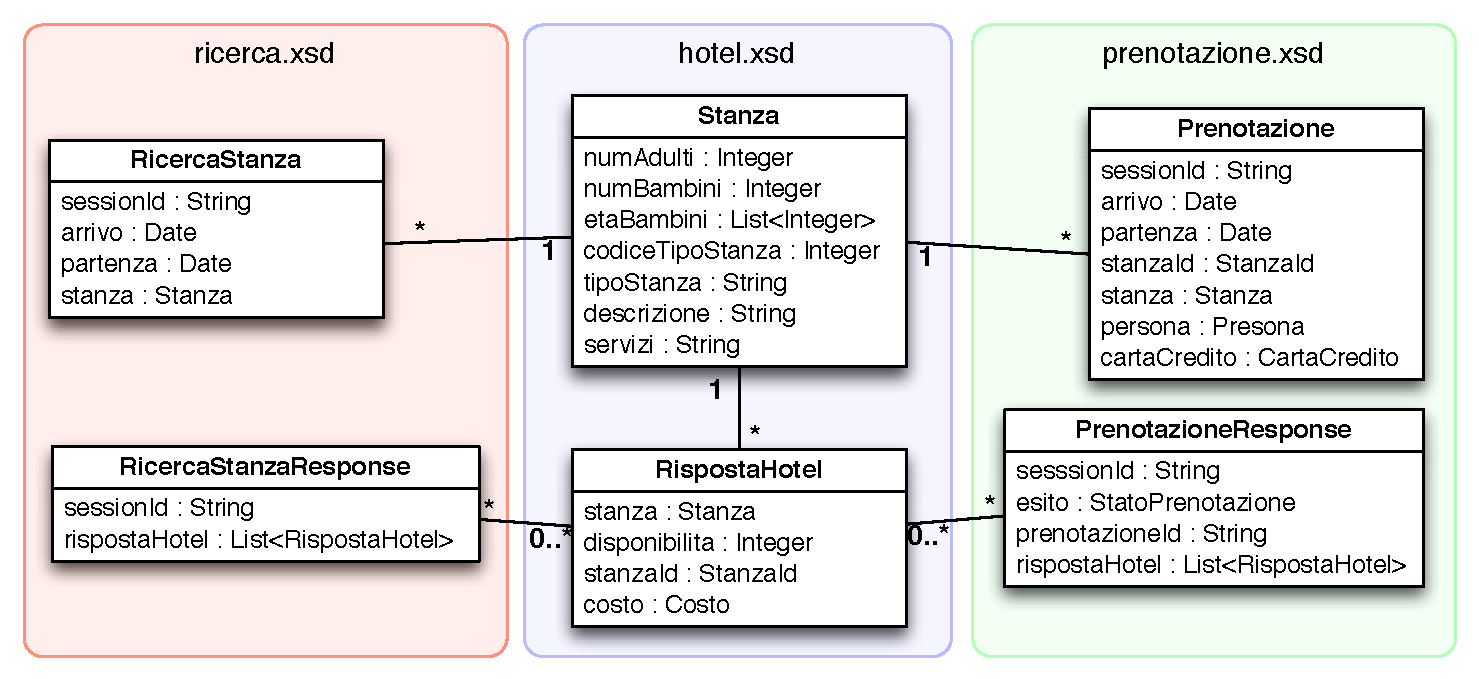
\includegraphics[scale = 0.58]{classi.pdf}
  \caption[asfd]{Rappresentazione grafica dei principali tipi definiti nei
    file XSD}
  \label{tipiXSD-figura}
\end{figure}

Per brevit\`a siano:\\
hotelns = ``http://www.hotel.com/hotel/'',\\
ricercans = ``http://www.hotel.com/ricerca/'', \\
prenotns = ``http://www.hotel.com/prenotazione/''.

Il tipo \verb'hotelns:stanza' descrive le proprit\`a di una camera
d'albergo come enunciato nella sezione~\ref{sec:descrizione}, non sono
presenti le propriet\`a della stanza proprie dell'hotel, quali
l'identificatore e il numero di stanze diponibili. La risposta ad un
messaggio di ricerca stanza \`e descritta dal tipo
\verb'ricercans:ricercaStanzaResponse' ed \`e costituita da una
sequenza di elementi di tipo \verb'hotelns:rispostaHotel'. Un elemento
di tipo \verb'hotelns:rispostaHotel' \`e una quatrupla costituita
dalla stanza, dall'identificatore usato dell'hotel per riferire la
stanza stessa, dalla disponibilit\`a effettiva della stanza nel
periodo di tempo indicato nella richiesta, e dal costo della stanza
stessa. Una sequenza di elementi \verb'hotelns:rispostahotel' pu\`o
essere presente anche nel messaggio di risposta alla prenotazione di
una stanza, \verb'prenotazione:prenotazioneRespo'\-\verb'nse', se la richiesta
di prenotazione \`e ambigua (non presenta l'identificatore
dell'hotel). In caso di prenotazione di una stanza registrata con
successo viene ritornato l'identificatore con il quale l'hotel ha
registrato la prenotazione, utilizzabile successivamente dal client
per verificare lo stato di prenotazione o cancellare la prenotazione. 

Ogni messaggio di richiesta inviato dal client pu\`o contentere un
elemento identificatore di sessione che consente al server di tenere
traccia delle operazioni eseguite da ogni singolo client.

%%%%%%%%%%%%%%%%%%%%%%%%%%%%%%%%%

\subsection{Esempi del contenuto XML nei messaggi SOAP}
Di seguito vengono presentati alcuni esempi di contenuti XML che
verificano i due schemi, ricerca.xsd e prenotazione.xsd.

\lstset{basicstyle=\small, tabsize=2, language=XML, breaklines=true,
  captionpos=b, frame=single} \lstinputlisting[firstline=2,
  rulecolor=\color{red},caption=ricerca di una
  stanza]{../xml_testFiles/ricerca1.xml} \lstinputlisting[firstline=2,
  rulecolor=\color{red}, caption=risposta alla ricerca di una
  stanza]{../xml_testFiles/soap_ricerca1-risposta.xml}
\lstinputlisting[firstline=2, rulecolor=\color{green},
  caption=prenotazione di una
  stanza]{../xml_testFiles/prenotazione1.xml}
\lstinputlisting[firstline=2, rulecolor=\color{green},
  caption={risposta che conferma, con stato pendente, la prenotazione
    di una stanza}]{../xml_testFiles/soap_prenotazione1-risposta2.xml}
\lstinputlisting[firstline=2, rulecolor=\color{green}, caption=altra
  risposta ad una prenotazione che mostra piu'
  alternative]{../xml_testFiles/soap_prenotazione1-risposta1.xml}

Tali esempi sono presenti nella directory
\verb'hotelBaseDir/xml_testFiles/' la validazione di questi pu\`o venir
effettuata con l'esecuzione di
\begin{verbatim}
$ java com.hotel.test.XmlTest -o test_validateXmlDocument
\end{verbatim}
con la variablile CLASSPATH opportuna.

%%%%%%%%%%%%%%%%%%%%%%%%%%%%%%%%%%%%%%%%%%%%%%%%%%%%%%%%%%%%%%%%%%%%%%%%%%%%%

\section{Note sulla realizzazione}
\subsection{Organizzazione dei sorgenti e delle risorse}
\label{sec:realizzazione.organizzazione}
Per la realizzazione del progetto si \`e utilizzato l'ambiente di
sviluppo \emph{Eclipse}, tutti i sorgenti e le risorse sono in
\verb+hotelBaseDir+, la base directory del progetto di eclipse, eccetto
le librerie usate (apache-cxf, servlet-api, etc ...).
\begin{description}
\item [build.xml] file \emph{Ant} con dei target per eseguire
  programmi clients e di test. Non vi sono target per la compilazione,
  eccetto per il programma client.
\item [doc/] doucmentazione e la relazione del progetto;
\item [hotel.war] l'archivio dei web service e della servlet Proxy
  pronto per il deploy in un Servlet Container.
\item [sources/java/] i sorgenti java del progetto, sia client side che
  server side;
\item [sources/resources/etc/] files di configurazione, in particolare i
  files properties di configurazione 
\item [sources/resources/keystore/] gli archivi java key store che
  contengono i certificati X.509 usati per realizzare la specifica
  WS-I;
\item [WebContent/] definizioni di schemi XML, descrizioni dei web
  services ;
\item [WebContent/WEB-INF/] configurazioni del servlet container e del
  framework Spring
\item [xml\_testFiles/] files xml per realizzare dei semplici test
  tramite programmi client quali \verb+curl+.
\end{description}
Tutti i sorgenti Java risiedono all'interno del package \verb'com.hotel'. I packages delle classi skeleton ricalcano i namespaces dei tre XSD, perci\`o:
\begin{itemize}
\item in com.hotel si hanno le classi che definiscono i tipi generali usati nell'applicazione,
\item in com.hotel.ricerca si hanno le classi per i tipi usati nelle operaizoni di ricerca,
\item in com.hotel.prenotaizone si hanno le classi per i tipi usati nelle operazioni di prenotazione.
\end{itemize}
Dato che i namespace dei due file WSDL cominciano con
http://www.hotel.com/ws/ allora si hanno i package
com.hotel.ws.ricerca e com.hotel.ws.prenotazione per le classi dei web
services ricerca e prenotazione.

La classe com.hotel.ws.PasswordCallback realizza il CallbackHandler
per ritirare la password del keystore dell'hotel, tale classe viene
utilizzata da entrambi i web service per firmare le risposte inviate
ai client.

Il programma cliente dell'applicazione, Client, ha package
com.hotel.client. In com.hotel.test vi sono alcuni test
sull'applicazione e su funzionalit\`a realizzate. In com.hotel.utils vi
sono classi che realizzano funzionalit\`a usate frequentemente.

\subsection{Implementazine del web service Ricerca}
\label{sec:realizzazione.ricerca}
Il web service descritto in WebContent/ricerca.wsdl \`e stato
realizzato con gestione manuale dei messaggi SOAP in ingresso e
uscita, tuttavia anche per tale file wsdl si \`e eseguito l'utility
\verb'wsdl2java' (senza l'argomento \verb'impl') creando le classi
java dei tipi utilizzati. Di tutte le classi skeleton create dai due
wsdl si sono definiti i costruttori per una migliore gestione
nell'implementazione dei web services. Anche
\verb'com.hotel.ws.ricerca.RicercaImpl' utilizza oggetti delle classi
skeleton, in quanto al momento dell'analisi del messaggio SOAP
ricevuto in ingresso, le informazioni ricavate vengono memorizzate in
oggetti di tali classi. La funzionalit\`a di ricerca di una stanza,
che interagisce con il database, viene realizzata con un metodo
pubblico e statico della classe RicercaImpl che riceve in ingresso e
ritorna oggetti delle classi skeleton; in tal modo tale funzionalit\`a
risulta usabile anche dal metodo prenotazione in
\verb'com.hotel.ws.prenotazione.PrenotazioneImpl'.


%%%%%%%%%%%%%%%%%%%%%%%%%%%%%%%%%%%%%%%%%%%%%%%%%%%%%%%%%%%%%%%%%%%%%%%%%%%%%

\section{Database}
\label{sec:database}
\lstset{basicstyle=\small, tabsize=2, language=SQL, breaklines=true,
  captionpos=b, frame=simple}

Il database dell'hotel contiene le tabelle descritte in
figura~\ref{fig:database}, per i dettagli sui tipi ed i vincoli di
foreign key si fa riferimento alla
sezione~\ref{sec:dettagli.database}. le colonne della tabella stanza
riflettono la descrizone data nella sezione~\ref{sec:descrizione}, in
particolare \verb'id' \`e come l'hotel identifica univocamente le
stanze, \verb'tipoStanza' \`e il codice che descrive la tipologia di
una stanza, tali codici sono uguali a quelli enumerati nella schema
xml hotel.xsd, la descrizione di tali codici \`e presente nella
tabella \verb'tipi_stanza'. 

\begin{figure}[h]
  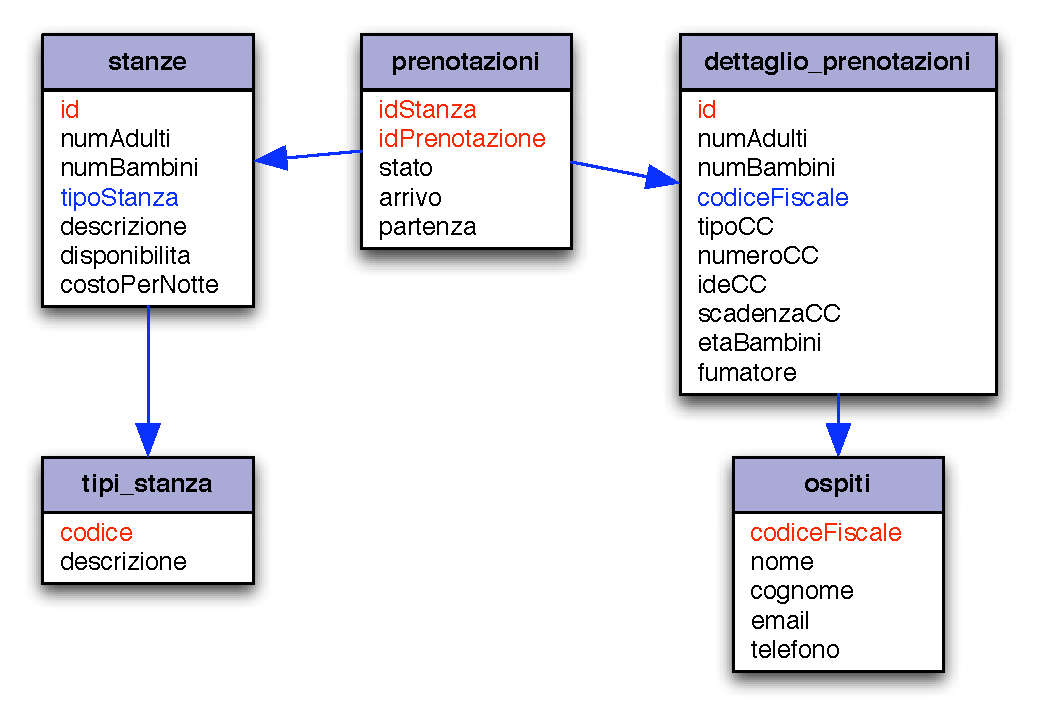
\includegraphics[scale=0.7]{tabelle.pdf}
  \caption{Tabelle del database}
  \label{fig:database}
\end{figure}

\subsection{Interazioni con il database}
\label{sec:database.interazioni}
Nel seguito viene descritto come sono realizzate le operazioni dei web
services e quali interrogazioni al database prevedono.

\subsubsection{Ricerca di una stanza}
I parametri in ingresso all'operazione di ricerca sono:
\begin{enumerate}
\item data di arrivo (es. \verb+2011-12-30+) e di partenza (es. \verb+2012-01-02+),
\item numero di adulti e numero di bambini (es. \verb+2+, \verb+2+). 
\item codice del tipo di stanza, non \`e obbligatorio (es. 1, st\`a
  per Suite Famiglia)
\end{enumerate}
L'operazione di ricercaStanza consiste nella ricerca, nella tabella
\verb'stanze' del database, delle camere d'albergo che soddifano i
parametri in ingresso \emph{2} e \emph{3}. Successivamente, per ogni
stanza che soddifa i vincoli imposti, si contano il numero di
prenotazioni che hanno un'intersezione non vuota con il periodo
temporale specificato nel parametro \emph{1}, tale valore \`e usato
per determinare l'effettiva disponibilit\`a di ogni stanza che
soddisfa la richiesta.

Le query eseguite sono:
\begin{lstlisting}
select * from stanze 
   where tipoStanza = 1 and numAdulti >= 2 and numBambini >= 2 ; 
\end{lstlisting}
Per ogni riga ritornata, sia ad esempio '1A0' il valore della colonna
\verb+id+, si esegue:
\begin{lstlisting}
select count(*) as numPrenotazioni from prenotazioni 
  where idStanza = '1A0' and (
    ( arrivo > '2011-12-30' and arrivo < '2012-01-02' ) or
    ( arrivo <= '2011-12-30' and partenza > '2011-12-30' )) ;
\end{lstlisting}
Il risultato fornisce il numero di prenotazioni della stanza '1A0'
durante il periodo di tempo specificato; tale valore va decrementato
alla disponibilit\`a totale della stanza stessa, il risultato viene
detto diponibilit\`a effettiva della stanza. Se la disponibilit\`a
effettiva di una stanza \`e maggiore di zero allora i dati della
stanza ottenuti dalla prima query vengono raccolti per essere
successivamente ritornati all'utente.

\subsubsection{Prenotazione di una stanza}
I parametri in ingresso all'operazione di prenotazione sono:
\begin{enumerate}
\item identificatore della stanza, fornito dall'hotel in una
  precedente ricerca di stanza (es. \verb+'1A0'+),
\item data di arrivo (es. \verb+'2011-12-30'+) e di partenza
  (es. \verb+'2012-01-02'+),
\item numero di adulti e numero di bambini (es. \verb+2+, \verb+2+) ed
  et\`a dei bambini (non necessaria),
\item credenziali del cliente: codice fiscale, nome, cognome,
  etc... (es. 'ASDFGHJ123456789', 'Federico', 'Mariti', ...),
\item tutte le informazioni sulla carta di credito (es. tipo='visa',
  numero='123', identificatore='123', scadenza='2013-04').
\end{enumerate}
Se l'identificatore della stanza non viene fornito l'operazione di
prenotazione agisce come la ricerca, lo stato di prenotazione
ritornato \`e nullo, \verb+NL+. Altrimenti si interroga il database
per ricavare il valore effettivo di disponibilit\`a della stanza nel
periodo di tempo specificato. 

Vengono eseguite le query per determinare la disponibilit\`a effettiva
della stanza identificata da \emph{1}:
\begin{lstlisting}
select disponibilita as disponibilita from stanze
    where id='1A0' ;

select count(*) numPrenotazioni from prenotazioni
    where idStanza = '1A0' and (
    ( arrivo > '2011-12-30' and arrivo < '2012-01-02' ) or
    ( arrivo <= '2011-12-30' and partenza > '2011-12-30' )) ;
\end{lstlisting}
Se \verb+disponibilita - numPrenotazioni+ \`e maggiore di zero allora
si procede con la prenotazione della stanza. Vengono effettuate query
in lettura sulle tabelle \verb'ospiti' e \verb'prenotazioni' per
determinare se il cliente \`e gi\`a registrato e quale sia
l'identificatore dell'ultima prenotazione registrata. Supponendo che
il cliente non sia registrato e che l'ultima prenotazione abbia
identificatore 'AA0003', vengono eseguite le seguenti query:
\begin{lstlisting}
insert into ospiti (codiceFiscale, nome, cognome) 
    values ('ASDFGHJ123456789', 'Federico', 'Mariti') ;

insert into dettaglio_prenotazioni (id, numAdulti, numBambini,
    codiceFiscale, tipoCC, numeroCC, ideCC, scadenzaCC) 
    values ('AA0004', 2, 2, 'ASDFGHJ123456789', 'visa', 123, 123,
        '2013-04') ;

insert into prenotazioni (idStanza, idPrenotazione, stato, arrivo,
    partenza)
    values ('1A0', 'AA0004', 'PD', '2011-12-30', '2012-01-02') ;
\end{lstlisting}

\subsection{Attacchi SQL injection}
\`E un tipo di attacco che si svolge invocando le funzionalit\`a del
sistema con parametri d'ingresso semanticamente non significativi, ma
creati ad arte per scoprire informazioni sulla struttura del database,
sul contenuto delle tabelle, ed anche per modificare il contenuto
delle tabelle. Tale attacco va a buon fine se le query, descritte
precedentemente, sono create come concatenazione di stringhe, ovvero i
parametri in ingresso ricevuti dal sistema sono trattati come stringhe
e concatenati tra loro per formare la query
compessiva. Nell'implementazione Java dei web services, ad ogni
interazione parametrica con il database, vengono usati oggetti della
classe java.sql.PreparedStatement per costruire le query da eseguire
nel database. Tutti i parametri della query, ricevuti in
ingresso, vengono interpretati e castati al rispettivo tipo prima di
essere compilati nella query tramite l'invocazione dei metodi setter
dell'oggetto PreparedStatement. Tale modo di procedere nega l'attacco
SQL injection.

\subsection{Problemi relativi alle transazioni concorrenti}
Nella sezione~\ref{sec:database.interazioni} sono state descritte le
query eseguite sul database per effettuare le operazioni di ricerca e
prenotazione di una stanza. In entrambi i casi viene eseguita una sola
transazione costituita dalle query descritte. Dato che il DBMS esegue
in modo concorrente le operazioni sottomesse da transazioni diverse,
ovvero, non \`e garantita la propriet\`a di isolamento delle
operazioni di una transazione, senza una adeguata gestione si possono
verificare comportamenti non coerenti con quelli attesi.

Si ipotizza che le uniche operazioni eseguite sul database siano
quelle di ricerca di una stanza e prenotazione di una stanza.

Si ipotizza che il DBMS realizzi la proprit\`a \emph{read safe
  transaction}, ovvero che la ricerca delle righe effettuata nelle
operazioni di una transazione veda unicamente gli aggiornamenti
consolidati, ovvero, effettuati da transazioni che sono state
committate.

Analiziamo la transazione della ricerca, prevede una lettura della
tabella \verb'stanze' e pi\`u letture della tabella
\verb'prenotazioni', tali letture sono riferite a sottoinsiemi
disgiunti di righe. L'esecuzione concorrente delle transazioni non
provoca particolari problemi. Non \`e possibile il fenomeno di
\emph{letture sporche} in quanto gli aggirnamenti non committati non
vengono considerati. \`E possibile leggere valori non corretti del
numero di prenotazioni di una certa stanza se dopo la lettura di tale
valore vengono committate una o pi\`u operazioni di prenotazione della
stessa stanza. Tuttavia i valori letti non vengono usati per
discriminare una scelta nella transazione, ma sono restituiti subito
all'utente\footnote{perci\`o possono diventare ``non corretti''
  durante l'esecuzione della ricerca come anche in un futuro non
  precisato. Per tale motivo non si \`e ritenuto necessario l'accesso
  in sola lettura alla tabella prenotazioni durante la
  ricerca.}. 

Analiziamo la transazione della prenotazione, prenvede la lettura
delle tabelle \verb'stanze' e \verb'prenotazioni' e la scrittura nelle
tabelle \verb'ospiti', \verb'dettaglio_prenotazione' e
\verb'prenotazione'. Le scritture sono effettuate solo se le
precedenti letture trovano la stanza richiesta per la prenotazione e
se la sua disponibilt\`a effettiva \`e maggiore di zero. \`E possibile
il verificarsi della \emph{perdita di aggiornamenti} sulla tabella
\verb'prenotazioni' se dopo la lettura del valore del numero di
prenotazioni della stanza vengono committate una o pi\`u prenotazioni
che hanno intersezione non vuota con il periodo temporale della
prenotazione. Ne segue che per una certa stanza e per un certo periodo
temporale possono venir registrate un numero di prenotazioni maggiore
della disponibilit\`a della stanza. Per evitare tale situalzione \`e
necessario imporre un vincolo di mutua esclusione nell'accesso in
scrittura alle tabelle coinvolte. Un modo di fare ci\`o nello standard
SQL \`e quello di imporre come \emph{livello di isolamento} il
\emph{Serializzable}.

%%%%%%%%%%%%%%%%%%%%%%%%%%%%%%%%%%%%%%%%%%%%%%%%%%%%%%%%%%%%%%%%%%%%%%%%%%%%%

\section{Dettagli sulla realizzazione}
\subsection{Proxy: uso di parametri iniziali}
Tale componente, realizzato da una Servlet, agisce da nodo intermedio
nelle comunicazioni SOAP tra i clients ed i web services. Per ogni web
service deve essere noto l'endpoint, la locazione dello schema XML e
l'insieme dei nomi che pu\`o assumere l'elemento wrapper nel soap:Body
(le operazioni). Anche se il problema considerato non prevede un
elevato numero di serivzi e di operazioni, si \`e deciso di risolvere
il problema della memorizzazione di tali informazioni in modo
generale, al fine di garantire una agevole modificabilit\`a ed
estensibilit\`a dell'applicazione.  Tali parametri vengono impostati
e/o aggiunti nel file \verb+web.xml+ senza conoscere (ne modificare)
l'implementazione della classe che realizza il proxy. I valori di tali
parametri vengono letti all'inizializzazione della Servlet che
realizza il proxy, estendendo il metodo \verb+init()+. Nel file
\verb+web.xml+ esistono, per la servlet \verb+Proxy+ tre parametri
iniziali: i nomi dei web services, gli endpoints, le locazioni degli
schemi; il valore di ogni parametro \`e composto da pi\`u
sottostringhe separate dal carattere 'spazio'; la prima sottostringa
in endpoints o in schemas \`e relativa alla prima sottostringa in web
services, e cos\`i via. Infine, per ciascun web service, i nomi delle
operazioni possibili sono specificate da un parametro il cui nome \`e
quello del web service seguito da ``-operations''.

In \verb+Proxy+ \`e stata definita una static-nested class,
\verb+Service+, che descrive un web service con i parametri menzionati
precedentemente. Durante l'inizializzazione della servlet viene
costruita un lista \footnote{synchronized} di \verb+Service+, tale oggetto
\`e usato nel metodo \verb+doPost+ della servlet per verificare se
l'operazione richiesta dal client \`e una di quelle accessibili,
validare tutto il contenuto della richiesta \footnote{solo se il
  contenuto della richiesta non \`e stato cifrato} ed inoltrare il
messaggio al web service corriposndente.

%%%%%%%%%%%%%%%%%%%%%%%%%%%%%%%%%

\subsection{Gestione manuale dei messaggi SOAP}

Come descritto nella sezione~\ref{sec:realizzazione.ricerca}, il
metodo \verb'invoke' della classe
\verb'com.hotel.ws.ricerca.Ricer'\-\verb'caImpl' gestisce manualmente i
messaggi SOAP. Il contentuto dei messaggi \`e salvato in memoria in
oggetti Java che rappresentano i tipi di dato possibili, quindi
vengono effettuate le operazioni su tali oggetti ed il risultato
restituito \`e nuovamente un oggetto Java che mappa un elemento del web
service. Le classi usate per questo scopo sono generate con l'utility
\verb'wsdl2java' ed hanno package come descritto nella
sezione~\ref{sec:realizzazione.organizzazione}.

Trasformare un elemento SOAP (si parte dal wrapper element, il figlio
del Body del messaggio SOAP), in un oggetto Java pu\`o essere fatto
iterando i figli dell'elemento, se un figlio non contiene elementi
SOAP allora il valore testuale viene settato nell'oggetto java grazie
ad una sequenza di \verb'if'-\verb'else' testando il nome del figlio,
altrimenti bisogna iterare anche il figlio ed ottenere l'oggetto Java
che rappresenti tale elemento, in tale oggetto verranno settati i
valori. Tuttavia si \`e ritenuto interessante realizzare un metodo
pi\`u generale ed espandibile (anche se il problema non lo
richiedeva). Si fa riferimeto alla documentazione realtiva al metodo
\verb'parseElementIn' e agli oggetti \verb'mappaSetter' e
\verb'mappaGetter' presenti nella classe \verb'RicercaImpl'.

%%%%%%%%%%%%%%%%%%%%%%%%%%%%%%%%%

\subsection{Database}
\label{sec:dettagli.database}
\lstset{basicstyle=\small, language=Clean, captionpos=b,
  frame=single, breaklines=true}

\begin{lstlisting}[caption=Tabelle]
 Schema |          Name          | Type  | Owner  
--------+------------------------+-------+--------
 public | dettaglio_prenotazioni | table | mariti
 public | ospiti                 | table | mariti
 public | prenotazioni           | table | mariti
 public | stanze                 | table | mariti
\end{lstlisting}

\begin{lstlisting}[caption={Tabella: Stanze}]
    Column     |          Type          | Modifiers 
---------------+------------------------+-----------
 id            | character varying(255) | not null
 numadulti     | smallint               | not null
 numbambini    | smallint               | not null
 tipostanza    | smallint               | not null
 descrizione   | character varying(255) | 
 disponibilita | smallint               | not null
 costopernotte | double precision       | not null
Indexes:
    ``stanze_pkey'' PRIMARY KEY, btree (id)
Foreign-key constraints:
    ``stanze_tipostanza_fkey'' FOREIGN KEY (tipostanza) REFERENCES tipi_stanza(codice)
Referenced by:
    TABLE ``prenotazioni'' CONSTRAINT ``prenotazioni_idstanza_fkey'' FOREIGN KEY (idstanza) REFERENCES stanze(id)
\end{lstlisting}

\begin{lstlisting}[caption={Tabella: prenotazioni}]
     Column     |          Type          | Modifiers 
----------------+------------------------+-----------
 idstanza       | character varying(255) | not null
 idprenotazione | character varying(255) | not null
 stato          | character varying(2)   | not null
 arrivo         | character varying(10)  | not null
 partenza       | character varying(10)  | not null
Foreign-key constraints:
    ``prenotazioni_idprenotazione_fkey'' FOREIGN KEY (idprenotazione) REFERENCES dettaglio_prenotazioni(id)
    ``prenotazioni_idstanza_fkey'' FOREIGN KEY (idstanza) REFERENCES stanze(id)
\end{lstlisting}

\begin{lstlisting}[caption={Tabella: dettaglio\_prenotazioni}]
    Column     |          Type          | Modifiers 
---------------+------------------------+-----------
 id            | character varying(255) | not null
 numadulti     | smallint               | not null
 numbambini    | smallint               | not null
 codicefiscale | character varying(16)  | 
 tipocc        | character varying(127) | not null
 numerocc      | smallint               | not null
 idecc         | smallint               | not null
 scadenzacc    | character varying(7)   | not null
 etabambini    | character varying(127) | 
 fumatore      | boolean                | 
Indexes:
    ``dettaglio_prenotazioni_pkey'' PRIMARY KEY, btree (id)
Foreign-key constraints:
    ``dettaglio_prenotazioni_codicefiscale_fkey'' FOREIGN KEY (codicefiscale) REFERENCES ospiti(codicefiscale)
Referenced by:
    TABLE ``prenotazioni'' CONSTRAINT ``prenotazioni_idprenotazione_fkey'' FOREIGN KEY (idprenotazione) REFERENCES dettaglio_prenotazioni(id)
\end{lstlisting}

\begin{lstlisting}[caption={Tabella: ospiti}]
    Column     |          Type          | Modifiers 
---------------+------------------------+-----------
 codicefiscale | character varying(16)  | not null
 nome          | character varying(255) | 
 cognome       | character varying(255) | 
 email         | character varying(255) | 
 telefono      | character varying(255) | 
Indexes:
    ``ospiti_pkey'' PRIMARY KEY, btree (codicefiscale)
Referenced by:
    TABLE ``dettaglio_prenotazioni'' CONSTRAINT ``dettaglio_prenotazioni_codicefiscale_fkey'' FOREIGN KEY (codicefiscale) REFERENCES ospiti(codicefiscale)
\end{lstlisting}

%%%%%%%%%%%%%%%%%%%%%%%%%%%%%%%%%

\subsection{Interazioni con il database per la prenotazione}
\lstset{basicstyle=\small, language=Java, captionpos=b,  frame=simple, breaklines=true}
\label{sec:dettagli.prenotazione}

L'operazione di prenotazione prevede una transazione che effettua
istruzioni di lettura e di scrittura dal/sul database. Dato che le
transazioni non sono eseguite in modo \emph{isolato} nel database,
allora questa transazione viene eseguita nella modalit\`a SQL
serializzable e si prevede una gestione esplicita delle politiche di
commit/rollback della stessa, al fine di evitare comportamenti
inattesi. L'implementazione segue lo schema proposto nel
codice~\ref{code:prenotazione}: eventuali conflitti di serializzazione
sono gestiti eseguendo l'istruzione SQL Rollback (che annulla tutti i
precedenti cambiamenti eseguiti nella transazione) e eseguendo
nuovamente tutte le istruzioni SQL della prenotazione.

\begin{lstlisting}[label={code:prenotazione}, caption={schema Java per la gestione dei conflitti di serializzazione}]
Connection con = null;
try {
  con = Database.getConnection(...);
  con.setTransaction(Connection.TRANSACTION_SERIALIZZABLE);
  con.setAutoCommit(false);
  boolean confilittiSerializzazione = false; 

  do {
    // letture sulle tabelle stanze e prenotazioni del database
    ...  = RicercaImpl.ricercaStanza(con, ...);
  
    if ( <stanza trovata e disponibile> ) {

      try { 
        // registra la prenotazione sul database
        <esegui INSERT sulle tabelle ospiti, dettaglio_prenotazioni, prenotazioni>;
        //consolida i cambiamenti effettuati sul database
        con.commit();

      } catch(SQLException e) {
        // annulla tutti i cambiamenti effettuati sul database
        con.rollback();

        if (e.getMessage().equals(``Could not serialize access due to concurrent update'')) {
          conflittiSerializzazione = true;
        } else {
          conflittiSerializzazione = false;
          ...
          throw new RuntimeException(e);
        }
      }
      
    } else {
      // camera non disponibile o prenotazione ambigua
      ...
    }

  } while(conflittiSerializzazione);

} catch(ClassNotFoundException e) {
  ...
} catch(SQLException E) {
  ...
} finally {
  con.close();
}
\end{lstlisting}

%%%%%%%%%%%%%%%%%%%%%%%%%%%%%%%%%

\subsection{Sicurezza}

La specifica WS-S viene ralizzata grazie al framework Spring, si fa
perci\'o riferimento alle seguenti configurazioni:
\begin{description}
\item [WebContent/WEB-INF/beans.xml] per il lato server,
\item [sources/java/com/hotel/client/beans.xml] per il client,
\item [sources/resources/etc/] le properties dei java key store,
\item [sources/resources/keystore/] i key store usati dal client e dal
  server.
\end{description}
L'hotel ha un keystore (\verb'hotel-keystore.jks') contenete una
coppia di chiavi RSA (l'alias \`e hotel) con cui firma i messaggi in
uscita. L'hotel fornisce il certificato autofirmato della sua chiave
pubblica, questo \`e archiviato in un altro keystore (con l'alias
hotel) usato dai clients per cifrare i messaggi in uscita e per
validare i messaggi in entrata.

%%%%%%%%%%%%%%%%%%%%%%%%%%%%%%%%%%%%%%%%%%%%%%%%%%%%%%%%%%%%%%%%%%%%%%%%%%%%%

\section{Esecuzione Client}
Vengono mostrati esempi di escuzione del programma client
dell'applicazione sviluppata in un sistema di tipo UNIX. 
Anzi tutto:
\begin{verbatim}
...
$ export CLASSPATH=$CP_HOTEL:$CP_CXF:$CP_CLI
$ java org.apache.axis.utils.tcpmon 2020 www.laiserver.com 8080 &
\end{verbatim}
si imposta la variabile d'ambinete CLASSPATH e si esegue un proxy che
esegue il forwarding dei dati tcp dalla porta 2020 sul localhost alla
porta 8080 dell'host in cui \`e deployata l'applicazione. Infatti in
fase di test il framework Spring usato dal programma client viene
istruito con indirizzi aventi macchina e porta pari a localhost e
2020, cos\`i da non mettere mano al file di configurazione di Spring
ogni volta che si vuole cambiare l'indirizzo dei servizzi, ma
semplicemente impostano un programma proxy. 

Per la riceca di una stanza si esegue:
\begin{verbatim}
$ java com.hotel.client.Client -b2011-12-30 -e2012-01-04 -a2 -c2
...
\end{verbatim}
o in modo equivalente, e pi\`u intuitivo:
\begin{verbatim}
$ java com.hotel.client.Client              \
> --arrivo 2011-12-30 --partenza 2012-01-04 \
> --numAdulti 2 --numBambini 2 
...
\end{verbatim}
Per la prenotazione si esegue:
\begin{verbatim}
$ java com.hotel.client.Client              \
> --arrivo 2011-12-30 --partenza 2012-01-04 \
> --numAdulti 2 --numBambini 2              \
> --etaBambini 7,12                         \
> --stanzaId 1A0                            \
> --persona \
ASDFGHJ123456789:Federico:Mariti:federico.mariti@gmail.com:0583123 \
> --cartaCredito visa:123:123:2012-05
\end{verbatim}

\end{document}
